 \documentclass[12pt,a4paper]{article}
%\usepackage{hyperref} % Use the Charter font for the document text
%\usepackage[UTF8]{ctex}
\usepackage{jheppub}

\usepackage{amsfonts,amssymb,amsmath}
\usepackage{mathtools}
\usepackage{tikz-cd}
\usepackage{tikz}
\usepackage{alltt}
\usepackage{amsfonts}
\usepackage{amsmath}
\usepackage{amssymb}
\usepackage{amsthm}
\usepackage{booktabs}
\usepackage{caption}
\usepackage{enumitem}
\usepackage{fancyhdr}
\usepackage{graphicx}
\usepackage{mathdots}
\usepackage{mathtools}
\usepackage{microtype}
\usepackage{multirow}
\usepackage{pdflscape}
\usepackage{pgfplots}
\usepackage{siunitx}
\usepackage{slashed}
\usepackage{tabularx}
\usepackage{tikz}
\usepackage{tkz-euclide}
\usepackage[normalem]{ulem}
\usepackage[all]{xy}
\usepackage{imakeidx}

\usepackage{wrapfig}

%%%今村セッテッティング%%%%%%%%%%%%%%%%%%%%%%%%%%%%%
\newcommand{\CC}{\mathbb{C}}
\newcommand{\ZZ}{\mathbb{Z}}
\newcommand{\RR}{\mathbb{R}}
\newcommand{\HH}{\mathbb{H}}

\newcommand{\hf}{\frac{1}{2}}
\newcommand{\tr}{{\rm tr}}
\newcommand{\ind}{{\rm ind}}
\newcommand{\ol}{\overline}
\newcommand{\ul}{\underline}
\newcommand{\up}{\uparrow}
\newcommand{\dn}{\downarrow}
\newcommand{\wt}{\widetilde}
\newcommand{\ra}{\rightarrow}
\newcommand{\wh}{\widehat}


%
%---------- mathbf font --------------------------------
%


\newcommand{\bfA}{\ensuremath{\mathbf{A}}}
\newcommand{\bfB}{\ensuremath{\mathbf{B}}}
\newcommand{\bfC}{\ensuremath{\mathbf{C}}}
\newcommand{\bfD}{\ensuremath{\mathbf{D}}}
\newcommand{\bfE}{\ensuremath{\mathbf{E}}}
\newcommand{\bfF}{\ensuremath{\mathbf{F}}}
\newcommand{\bfG}{\ensuremath{\mathbf{G}}}
\newcommand{\bfH}{\ensuremath{\mathbf{H}}}
\newcommand{\bfI}{\ensuremath{\mathbf{I}}}
\newcommand{\bfJ}{\ensuremath{\mathbf{J}}}
\newcommand{\bfK}{\ensuremath{\mathbf{K}}}
\newcommand{\bfL}{\ensuremath{\mathbf{L}}}
\newcommand{\bfM}{\ensuremath{\mathbf{M}}}
\newcommand{\bfN}{\ensuremath{\mathbf{N}}}
\newcommand{\bfO}{\ensuremath{\mathbf{O}}}
\newcommand{\bfP}{\ensuremath{\mathbf{P}}}
\newcommand{\bfQ}{\ensuremath{\mathbf{Q}}}
\newcommand{\bfR}{\ensuremath{\mathbf{R}}}
\newcommand{\bfS}{\ensuremath{\mathbf{S}}}
\newcommand{\bfT}{\ensuremath{\mathbf{T}}}
\newcommand{\bfU}{\ensuremath{\mathbf{U}}}
\newcommand{\bfV}{\ensuremath{\mathbf{V}}}
\newcommand{\bfW}{\ensuremath{\mathbf{W}}}
\newcommand{\bfX}{\ensuremath{\mathbf{X}}}
\newcommand{\bfY}{\ensuremath{\mathbf{Y}}}
\newcommand{\bfZ}{\ensuremath{\mathbf{Z}}}
\newcommand{\bfa}{\ensuremath{\mathbf{a}}}
\newcommand{\bfb}{\ensuremath{\mathbf{b}}}
\newcommand{\bfc}{\ensuremath{\mathbf{c}}}
\newcommand{\bfd}{\ensuremath{\mathbf{d}}}
\newcommand{\bfe}{\ensuremath{\mathbf{e}}}
\newcommand{\bff}{\ensuremath{\mathbf{f}}}
\newcommand{\bfg}{\ensuremath{\mathbf{g}}}
\newcommand{\bfh}{\ensuremath{\mathbf{h}}}
\newcommand{\bfi}{\ensuremath{\mathbf{i}}}
\newcommand{\bfj}{\ensuremath{\mathbf{j}}}
\newcommand{\bfk}{\ensuremath{\mathbf{k}}}
\newcommand{\bfl}{\ensuremath{\mathbf{l}}}
\newcommand{\bfm}{\ensuremath{\mathbf{m}}}
\newcommand{\bfn}{\ensuremath{\mathbf{n}}}
\newcommand{\bfo}{\ensuremath{\mathbf{o}}}
\newcommand{\bfp}{\ensuremath{\mathbf{p}}}
\newcommand{\bfq}{\ensuremath{\mathbf{q}}}
\newcommand{\bfr}{\ensuremath{\mathbf{r}}}
\newcommand{\bfs}{\ensuremath{\mathbf{s}}}
\newcommand{\bft}{\ensuremath{\mathbf{t}}}
\newcommand{\bfu}{\ensuremath{\mathbf{u}}}
\newcommand{\bfv}{\ensuremath{\mathbf{v}}}
\newcommand{\bfw}{\ensuremath{\mathbf{w}}}
\newcommand{\bfx}{\ensuremath{\mathbf{x}}}
\newcommand{\bfy}{\ensuremath{\mathbf{y}}}
\newcommand{\bfz}{\ensuremath{\mathbf{z}}}




%%%横山セッティング%%%%%%%%%%%%%%%%%%%%%%%%%%%%%%%%%
\newcommand{\NN}{\mathcal{N}\!}
\newcommand{\DD}{\mathcal{D}}
\newcommand{\UU}{U(1)}
\newcommand{\dd}{\mathrm{d}}
\renewcommand{\SS}{\mathbf{S}}
\renewcommand{\Im}{\mathrm{Im}}
\renewcommand{\Re}{\mathrm{Re}}
%\renewcommand{\<}{\langle}
\renewcommand{\>}{\rangle}
\newcommand{\Tr}{{\rm Tr}}

\renewcommand{\r}{\mathrm}

\newcommand{\sign}{\mathrm{sign}}

\newcommand{\lra}{\leftrightarrow}
\newcommand{\LL}{\mathcal{L}}
\newcommand{\la}{\leftarrow}
\newcommand{\ro}{\sqrt}
\newcommand{\Ra}{\Rightarrow}
\newcommand{\Pexp}{\mathrm{Pexp}}

\newcommand{\nn}{\nonumber \cr}
%\newcommand{\1}{\mbox{1}\hspace{-0.25em}\mbox{l}}

%数字のみ対応
\newcommand{\Maru}[1]{\ooalign{
\ifnum#1<10 \hfil\resizebox{.9\width}{.85\height}{#1}\hfil
\else
\hfil\resizebox{.6\width}{.8\height}{#1}\hfil
\fi
\crcr
\raise.1ex\hbox{$\bigcirc$}}}

%全文字対応
\newcommand{\maru}[1]{\ooalign{
\hfil\resizebox{.8\width}{\height}{#1}\hfil
\crcr
\raise.1ex\hbox{\large$\bigcirc$}}}


\newcommand{\nord}[1]{\vcentcolon\mathrel{#1}\vcentcolon}
\providecommand{\vcentcolon}{\mathrel{\mathop{:}}}


\def\P{\mathop{\cal P}}
\def\diag{\mathop{\rm diag}}


\def\Re{\mathop{\rm Re}\nolimits}
\def\Im{\mathop{\rm Im}\nolimits}
\def\Det{\mathop{\rm Det}\nolimits}
\def\sign{\mathop{\rm sign}\nolimits}


%%% rap %%% - make two letters overlap
\newcommand{\rap}[2]
{\setbox1=\hbox{#1}%
\setbox2=\hbox to\wd1{\hss #2\hss}%
\mbox{\rlap{\box1}\box2}}

%\newcommand{\sla}[1]{\rap{$#1$}{/}}
\newcommand{\sla}[1]{\rap{$#1$}{$\backslash$}}


\def\DY#1{{\MyGreen [DY: #1]}}
\newcommand{\MyGreen}{\color [rgb]{0,0.7,0}}

\usepackage[vcentermath]{youngtab}
% \Yboxdim4pt
\newcommand{\Y}{\yng}
\newcommand{\Young}{}


%    \renewcommand*{\bm}[1]{#1}%
%    % any other necessary redefinitions 


%%%title def%%%%%%%%%%%%%%%%%%%%%%%%%%%%%%%%%%%%%%%%%%%%%%%

\makeatletter
\def\maketitle{
\noindent
{\Large \@title \par\vskip 2pt}
\noindent
{\large \@date \hspace{4pt} \@author}
%\cr[-2pt]
%\noindent------------------------------------------------------------------------------------------
\par\vskip 1.5em
}

\author{横山 大輔}
\date{\today}
%%%本文%%%%%%%%%%%%%%%%%%%%%%%%%%%%%%%%%%%%%%%%%%%%%%%%%%%%%%%%

% \title{\centerline{Lecture 2}}
\begin{document}
% \maketitle
% \begin{abstract}

% \end{abstract}
% \tableofcontents

  \pagestyle{fancy}
  \renewcommand{\headrulewidth}{0.0pt}
  \rhead{}
  \lhead{}
  \cfoot{[\ \scshape\oldstylenums{\thepage}\ / %
    \scshape\oldstylenums{\pageref{lastpage}} ]}
    
%  \rfoot{\@author}

% \setcounter{section}{}
% \setcounter{subsection}{}
% \setcounter{subsubsection}{}

\centerline{\Large \bf  Lecture 8}

\vspace{12pt}
% \DY{なにかコメント}

\vspace{-12pt}




\section{Introduction for D-brane}
% \DY{昔$p^\mu$が保存していないことを見てい
% るので、それから D-brane を導入する?}
% \DY{Boundary condition から D-brane を導入する?}
% \DY{Closed string theory は consistent.}


Physical problem of the oriented closed superstring theories (IIA, IIB) is
a lack of gauge fields.
On the other hand, we already know a gauge field appears from open string.
Let us look into an open string further,
then, we will see that open string needs an object, so called \textrm{D-brane}.


% What we will learn in this lecture.
% \begin{itemize}
%  \item Notion of D-brane
%  \item Chan-Paton factor and (unitary) gauge group
% \end{itemize}


% What we will NOT learn in this lecture, but in following lectures.
% \begin{itemize}
%  \item Action \& Tension
%  \item Spectrum \& Amplitude (vacuum, one-loop)
%  \item Their features (bound-states, etc.)
% \end{itemize}


% What we will NOT learn in this course.
% \begin{itemize}
%  \item CFT with boundary
% \end{itemize}

Note that closed superstring theories are consistent by itself.
However, only open string theory is inconsistent,
and it needs closed string as well (see Fig.~\ref{OpenClosed.eps}).
\begin{figure}[htb]
\centerline{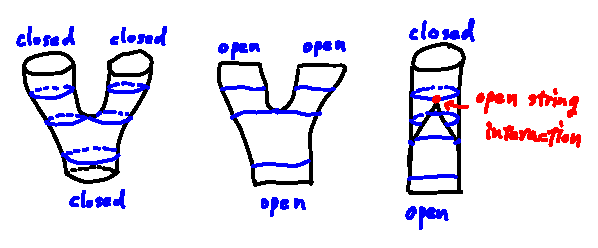
\includegraphics[width=350pt]{OpenClosed.eps}}
\caption{Open string interaction induces closed string}
\label{OpenClosed.eps}
\end{figure}

\subsection{Boundary conditions \& D-brane}

Let us consider an open string action.
\begin{align*}
 S_\mathrm{E} = \frac{1}{4\pi \alpha'} \int_{\sigma=0}^{\sigma=\pi} dtd\sigma
 \left( \partial_t X \cdot \partial_t X +\partial_\sigma X \cdot \partial_\sigma X  \right) \ ,
\end{align*}
where the subscript $E$ shows the world-sheet(WS) is Euclidean.
The variation principle leads
\begin{align*}
 0 &= \delta S
 = \frac{1}{2\pi \alpha'} \int_{\sigma=0}^{\sigma=\pi} dtd\sigma
 \left( \partial_t X \cdot \partial_t \delta X +\partial_\sigma X \cdot \partial_\sigma \delta X  \right)  \nonumber\\
 &= \frac{1}{2\pi \alpha'} \int_{\sigma=0}^{\sigma=\pi} dtd\sigma
 \left[ -\delta X \cdot \left( \partial_t \partial_t X +\partial_\sigma \partial_\sigma X \right)
 + \partial_t\left(\partial_t X \cdot \delta X \right) + \partial_\sigma \left( \partial_\sigma X \cdot\delta X \right)  \right]  \nonumber\\
 &= \frac{1}{2\pi \alpha'} \int dt \left[ \partial_\sigma X \cdot\delta X  \right]_{\sigma=0}^{\sigma=\pi} \ .
\end{align*}
At the last equality we used E.O.M and $\delta X (t=\pm \infty)=0$.
The equation compels us to impose one of either boundary conditions:
\begin{align*}
 \begin{array}{ll}
  \partial_\sigma X^\mu |_\mathrm{bdy} = 0 \qquad &\textrm{Neumann condition}  \\[4pt]
  \delta X^\mu |_\mathrm{bdy} = 0 \textrm{ or } X^\mu = c^\mu \ (\mathrm{const}) \qquad &\textrm{Dirichlet condition}
 \end{array}
\end{align*}


From the homework 1 we saw that the solution for Dirichlet boundary condition
express a momentum NON-conservation (see Fig.~\ref{BoundaryObj.eps}).
\begin{figure}[htb]
\centerline{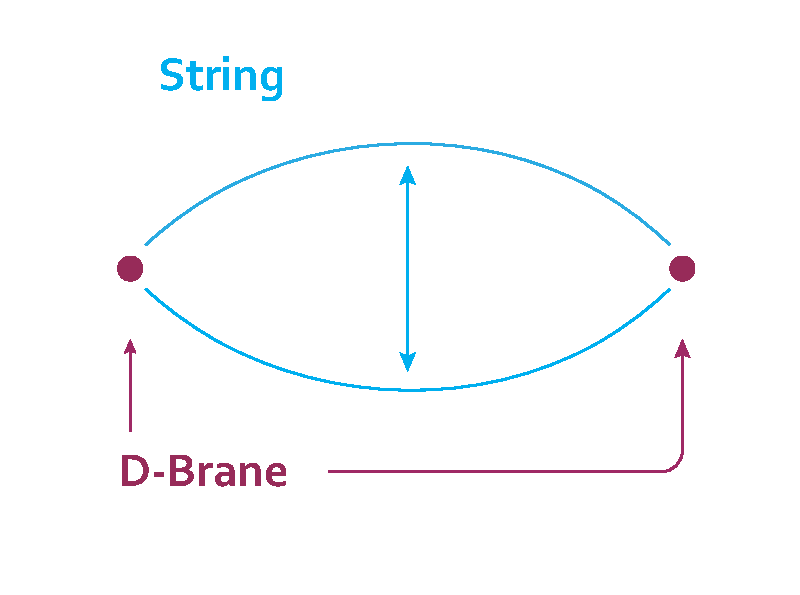
\includegraphics[width=100pt]{BoundaryObj.eps}}
\caption{D-brane must exist at the ends of open string so that momentum can escape from string.}
\label{BoundaryObj.eps}
\end{figure}
It implies that there must be something into which the momentum goes.
We call this object \textbf{D-brane}, where the D stands for Dirichlet and
brane comes from membrane.
D-brane is a dynamical object as it should receive the momentum,
hence, it has action and interactions with string.
On the other hand, in order to stay at a specific point $X^\mu = c^\mu$
D-brane must be infinitely heavy compared to string.


One can impose a certain number of Neumann condition and the rest is Dirichlet, let us set:
\begin{align*}
 &\textrm{Neumann condition on } X^a \quad (a=0,1,\cdots,p)  \\
 &\textrm{Dirichlet condition on } X^I \quad (I=p+1,\cdots,D-1)
\end{align*}
The corresponding D-brane is called D$p$-brane (e.g. D3-brane).
\textbf{D$p$-brane} is a spacially $p$-dim object and space-timely $(p+1)$-dim object.
Now we can visalize a configuration of D-brane and string as in Fig.~\ref{DpBrane.eps}.
\begin{figure}[htb]
\centerline{\includegraphics[width=150pt]{DpBrane.eps}}
\caption{Visalization of D$p$-brane and open string.}
\label{DpBrane.eps}
\end{figure}



\subsection{Chan-Paton factor}

We can consider not only a D-brane but many D-branes,
and a string now have an option on which D-brane a string ends.
Let us label this option $i$ ($i=1,\cdots,n$), which is called \textbf{Chan-Paton factor}.
As an open string has two end points a string state has two Chan-Paton degree:
\begin{align*}
 |N;k \rangle  \quad  \to \quad |N;k;ij \rangle \ .
\end{align*}
Now we have $n^2$ massless vector states in both bosonic- or super-string theory.
As usual we use $n \times n$ Hermite matrices $T^a$ normalized to
\begin{align*}
 \tr (T^a T^b) = \delta^{ab} \ ,
\end{align*}
which is a complete set for the end points:
\begin{align*}
 |N;k;a \rangle = T^a_{ij} |N;k;ij \rangle \ .
\end{align*}
You will find this is $U(n)$ gauge fields
if you compute a three point amplitude.



Note that in order to realize $U(n)$ gauge group the D-branes must coincide at a point.
Otherwise, the gauge group is broken by Higgs mechanism (see Fig.~\ref{ManyD.eps}).
\begin{figure}[htb]
\centerline{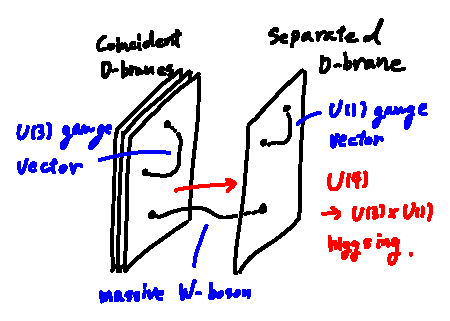
\includegraphics[width=250pt]{ManyD.eps}}
\caption{Many D-branes and Chan-Paton factors. $U(n)$ gauge group and Higgs mechanism.}
\label{ManyD.eps}
\end{figure}


We will see, in next lectures, that other type of gauge groups ($SO$ or $Sp$) can be realized in string theory.



\subsection{D-brane in IIA/IIB superstring theory}


In the previous lecture note we saw that IIA/IIB superstring theory has RR fields,
which are anti-symmetric tensors and are analogy of gauge fields.
Furthermore, again from an analogy of electro-magnetic dynamics,
there are objects which electrically/magnetically coupled to the gauge fields
like an electron/monopole.
It is known that for RR fields such objects are D-branes.
In order to justify the statement we need more elaborated tools.
Here we simply see that which D$p$-branes couple to RR fields in IIA/IIB.


Let us start with an electron/monopole in 4-dim spacetime.
Electron is expressed by a source
$J^\mu = (\rho, \bfj) = (q \delta^3(\bfr-\bfr(t)), \partial_t \bfr(t) \rho )$
and its coupling to gauge field is written by
\begin{align*}
 S_J = q \int A_\mu J^\mu d^4x = q \int_C A_\mu dx^\mu = q \int_C A \ ,
\end{align*}
where $q$ is an electric charge, $C$ is a worldline of the electron, and $A$ is understood as 1-form.
Similarly, D$p$-brane ($p\le 3$) couples to $(p+1)$-tensor RR field as follows.
\begin{align*}
 S_{Dp} = \int_{M_{p+1}} C_{p+1} \ ,
\end{align*}
where $C_{p+1}$ is a $(p+1)$-form RR gauge potential
and $M_{p+1}$ is a world-membrane of D$p$-brane.
Note that an exteriror deribative of the potential
gives its field strength $G_{p+1} = d C_p$.
For example of D$3$-brane is:
\begin{align*}
 S_{D3} &= \int_{M_{4}} C_{4} = \frac{1}{4!} \int_{M_{4}} C_{\mu\nu\rho\sigma}
 dX^\mu \wedge dX^\nu \wedge dX^\rho \wedge dX^\sigma  \nonumber\\
 &= \frac{1}{4!} \int_{M_{4}} C_{\mu\nu\rho\sigma} \epsilon^{abcd}
 \frac{\partial X^\mu}{d\sigma^a} \frac{\partial X^\nu}{d\sigma^b}
 \frac{\partial X^\rho}{d\sigma^c} \frac{\partial X^\sigma}{d\sigma^d} d^4\sigma \ ,
\end{align*}
where $\sigma^a$ is a world-sheet coordinate of D$3$-brane and $X^\mu$
is an embeding of D$3$-brane into space-time.
The reason why it is limited up to $p=3$ is because
we only have up to $4$-tensor RR-field in IIA/IIB superstring theory.


% Monopole cannot be expressed by fundamental particle,
% rather it is a solitonic object, which is expressed by a field configuration.
Monopole is characterized by maginetic flux measured at surface surrounding the monopole
(see Fig.~\ref{mono.eps})
\begin{figure}[htb]
\centerline{\includegraphics[width=150pt]{mono.eps}}
\caption{Monopole is measured by magnetic flux configuration.}
\label{mono.eps}
\end{figure}
\begin{align*}
 q_m &= \int_S B \cdot n dS = \int_{B_3} \nabla \cdot B dV \ , \\
 &= \int_{\partial B} F_2 = \int_{B} dF_2 \ ,
\end{align*}
where $q_m$ is a magnetic charge, $B$ is magnetic flux, $S$ is a surface surrounding
the monopole, $B_3$ is a 3-dim ball, whose boundary is $S$,
$B$ in the second line is $B_3$, and $\partial B$ is a surface of $B$, which is $S$.
Note that $F_2$ cannot be expressed by an exterior derivative $dA$ globally,
hence, $dF_2 \neq 0$, rather $dF_2 = \nabla \cdot B = q_m \delta^3(r)$.
If we extend this idea to D$p$-brane ($p \ge 3$)
\begin{align*}
 q_m &= \int_{\partial B_{D-(p+1)}} G_{D-(p+2)} = \int_{B_{D-(p+1)}} dG_{D-(p+2)} \ .
\end{align*}
See Fig.~\ref{MagD.eps} to understand the direction of the flux $G_{D-(p+2)}$,
which leads potential $C_{D-(p+3)}$.
The reason why $p \ge 3$ is because $D=10$ and the highest tensor is $[4]$.
\begin{figure}[htb]
\centerline{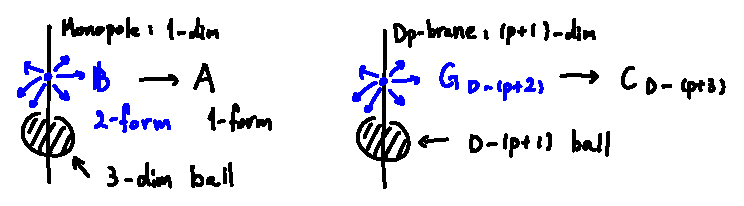
\includegraphics[width=350pt]{MagD.eps}}
\caption{Higher dimensional analog of monopole: magnetically coupled D$p$-brane.}
\label{MagD.eps}
\end{figure}

If you allow to use electro-magnetic duality it is more easily understood (see Fig.~\ref{EleMagD.eps}).
\begin{figure}[htb]
\centerline{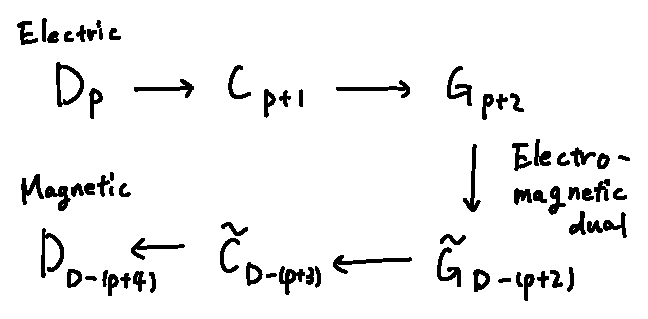
\includegraphics[width=250pt]{EleMagD.eps}}
\caption{Electro-magnetic duality and D-brane.}
\label{EleMagD.eps}
\end{figure}

String or fundamental string, denoted as F$1$, is electrically coupled to B-field.
On the other hand, there is an object that is magnetically coupled to B-field,
which is called \textbf{NS$5$-brane}.


Now you should notice that in IIA/IIB string theory the number $p$ of D$p$-brane
is limited to a certain number.
This is because the rank of RR-field (tensor) is limited.
Let us summarize which D-brane can exist in which superstring theory (see Table~\ref{table:001}).
\begin{table}[htbp]
 \centering{
  \caption{Possible D-branes in IIA/IIB superstring, fundamental string, and NS$5$-brane.}
  \vspace{4pt}
  \label{table:001}
\begin{tabular}{l|ccc}
  IIA & $B_2$ & $C_1$ & $C_3$ \\
\hline
  Electric & F$1$ & D$0$ & D$2$ \\
  Magnetic & NS$5$ & D$6$ & D$4$ \\
\end{tabular} \hspace{12pt}
\begin{tabular}{l|cccc}
  IIB & $B_2$ & $C_0$ & $C_2$ & $C_4^+$ \\
\hline
  Electric & F$1$ & D$(-1)$ & D$1$ & D$3$ \\
  Magnetic & NS$5$ & D$7$ & D$5$ & D$3$ \\
\end{tabular}
}
\end{table}
\vspace{2pt}
\noindent
\textbf{Comments:}\vspace{-2pt}
\begin{itemize}
 \item Only D$p$-brane for even $p$ exist in IIA and for odd $p$ in IIB.
 \item D$(-1)$-brane is timely localized object (like instanton).
 \item D$8$-brane can exist in IIA, which is a non-dynamical object
       and there is no corresponding anti-symmetric tensor.
\end{itemize}







\section{1-loop amplitude}


We continue to study amplitude, here it is 1-loop amplitude.
1-loop amplitude is important because
it includes quantum information, such as anomaly.



% \DY{UV finite であることを説明したい。}

\subsection{Torus and its modulus \& CKG}

Here, we will briefly see $g=1$ case, which is nothing but torus.
Torus can be constructed from 1d flat complex space $\CC$ by identification (see Fig.~\ref{torus.eps})
\begin{figure}[htb]
\centerline{\includegraphics[width=150pt]{torus.eps}}
\caption{Torus from $\CC$ by the identification.}
\label{torus.eps}
\end{figure}
\begin{align*}
 z \sim z+2\pi \sim z+2\pi \tau \ ,
\end{align*}
where $\tau = \tau_1 +i\tau_2$ and assume $\tau_2 > 0$.
Since the metric is flat the $\tau$ is a complex modulus, which describe the ``shape'' of the torus.
There is also a complex translation invariance, which is 2 CKG.

Torus has so called a \textbf{modular invariance}.
Let us define two generators:
\begin{align*}
 T: \tau \to \tau+1 \ , \quad S: \tau \to -\frac{1}{\tau} \ .
 \label{eq:ModularTra}
\end{align*}
These $T,\ S$ generates modular transformation
\begin{align*}
 \tau \to \frac{a\tau+b}{c\tau+d} \ , \quad
 \begin{pmatrix}
  a & b \\ c & d
 \end{pmatrix} \in PSL(2,\ZZ) \ ,
\end{align*}
The ``shape'' of torus is conformally invariant under the modular transformation.
Therefore, the parameter space of $\tau$ is limited to the fundamental region, see Fig.~\ref{fundamental.eps}.
\begin{figure}[htb]
\centerline{\includegraphics[width=120pt]{fundamental.eps}}
\caption{Fundamental region of $\tau$.}
\label{fundamental.eps}
\end{figure}

As we did for sphere case we will encounter ghost expectation,
whose contribution is only from the zero modes.
In the torus case since the space is flat and finite,
we can insert a WS integral as follows
\begin{align*}
 \langle c(0) \rangle_{bc} = \langle C \rangle_{bc} \ , \quad C \equiv \int \frac{d^2z}{4\pi^2\tau_2}c(z) \ .
\end{align*}
($\ol C$ and $B, \ol B$ are similarly defined.)


The string amplitude for torus case is
\begin{align*}
 A_{1,n}
 &= g_\textrm{st}^{n} \frac{1}{2} \int_F d^2\tau   \left\langle (b, \partial_\tau h) (b, \partial_{\ol\tau} h)
 c\ol c\ \sqrt h V_1 \prod_{j=2}^{n}\int d^2z_j \sqrt h V_j \right\rangle \ .
\end{align*}
As the same logic as before we can insert the integration even for $z_1$ since the amplitude should not depend on $z_1$:
\begin{align*}
 A_{1,n}
 &= g_\textrm{st}^{n} \frac{1}{2} \frac{1}{4\pi^2\tau_2} \int_F d^2\tau
 \left\langle (b, \partial_\tau h) (b, \partial_{\ol\tau} h) C\ol C\ \right\rangle_{bc}
 \left\langle \prod_{j=1}^{n}\int d^2z_j \sqrt h V_j \right\rangle_X \ .
\end{align*}


Though seemingly the metric would not depend on $\tau$, it does indeed depend on $\tau$ as follows.
Let us consider small deformation of the metric
\begin{align*}
 &ds^2 = dzd\ol z \to d(z+\epsilon\ol z) d(\ol z+\ol\epsilon z) \ , \\
 &\Leftrightarrow \quad \delta h_{zz} = \ol\epsilon \ , \quad \delta h_{\ol z\ol z} = \epsilon \ .
\end{align*}
New torus has coordinate $z+\epsilon \ol z$.
This deformation changes the period to $(2\pi (1+\epsilon),2\pi(\tau+\epsilon\ol\tau))$.
Therefore the modulus becomes $\wt \tau = \frac{\tau+\epsilon\ol\tau}{1+\epsilon} \simeq \tau -2i\epsilon\tau_2$
$\Leftrightarrow\ \delta \tau = -2i\epsilon\tau_2$.
Now the $\tau$ derivative is
\begin{align*}
 \partial_\tau h_{\ol z\ol z} = \lim_{\epsilon \to 0} \frac{\delta h_{\ol z\ol z}}{\delta \tau} = \frac{i}{2\tau_2} \ ,
 % \quad \partial_{\ol \tau} h_{zz} = -\frac{i}{2\tau_2} \ ,
 \quad\Rightarrow\quad (b, \partial_\tau h) = 2\pi i B \quad \textrm{etc} \ ,
\end{align*}
where
\begin{align*}
 (b, \partial_\tau h) = \int \frac{d^2z}{4\pi} \sqrt{h}\ b_{ab} \frac{\partial}{\partial \tau}  h^{ab}(\tau) \ .
\end{align*}

\subsection{Torus partition function for bosonic string}

One may think the simplest amplitude would be tachyon amplitude,
however, it is actually vacuum amplitude $n=0$, which can be calculated in torus case opposed to sphere case.
\begin{align*}
 A_{1,0}
 &= \frac{1}{2} \int_F \frac{d^2\tau}{\tau_2}
 \left\langle B\ol B C\ol C\ \right\rangle_{bc}
 \left\langle 1 \right\rangle_X \ .
\end{align*}


\subsubsection*{Matter sector}

Using operator formalism
\begin{align*}
 \left\langle 1 \right\rangle_X = \tr \exp \left[ 2\pi i \left( \tau_1 P +i\tau_2 H \right)\right]
 = \tr \left[ q^{L_0 -\frac{c}{24}} \ol q^{\ol L_0 -\frac{c}{24}} \right] \ ,
\end{align*}
where $q = e^{2\pi i\tau}$, $P = L_0 -\ol L_0$, $H = L_0 +\ol L_0 -\frac{c}{12}$, and
\begin{align*}
 L_0 = \frac{\alpha'}{4} p^2 +\sum_{n > 0} \alpha_{-n} \cdot \alpha_n \ .
\end{align*}
Note that $e^{-2\pi \tau_2 H}$ is a thermal factor or Euclideanized time translation,
and $e^{2\pi i \tau_1 P}$ is a space translation.
The result is (homework)
\begin{align*}
 \left\langle 1 \right\rangle_X &=
 \int \frac{d^Dxd^Dp}{(2\pi)^D} \exp \left( -4\pi\tau_2 \frac{\alpha'}{4} p^2 \right)
 \left| \frac{q^{-\frac{1}{24}}}{\prod_{n \ge 1} (1-q^n)} \right|^{2D}  \nonumber\\
 &= i \frac{V_{26}}{(2\pi l_s)^{26}} \left(\tau_2\right)^{-13} \left|\eta(\tau)\right|^{-52} \ ,
\end{align*}
where $l_s = \sqrt{\alpha'}$, and $\eta(\tau)= q^{\frac{1}{24}} \prod_{n=1}^\infty (1-q^n)$.
$i$ in the second line is from Wick-rotation of space-time momentum $p^0 \to ip^0_E$,
which is needed to define Gaussian integral.


\subsubsection*{Ghost sector}


Similarly,
\begin{align*}
 \left\langle B\ol B C\ol C\ \right\rangle_{bc}
 = \tr \left[ (-1)^F b_0 \ol b_0 c_0 \ol c_0 q^{L_0 -\frac{c}{24}} \ol q^{\ol L_0 -\frac{c}{24}}  \right]
\end{align*}
with
$c=-26$ and $L_0 = \sum_{n \in \ZZ} (n \nord{b_{-n}c_n}) -1$.
$F$ is a fermion number operator; $F=1$ for fermion and $F=0$ for boson,
and hence, $(-1)^F$ anti-commutes with fermions and commutes with boson.
The eigenvalue of $(-1)^F$ for a vacuum depends on the situation;
usually it is $+1$, namely, $(-1)^F |0\rangle = |0\rangle$.
However, there is an example gives minus sign as we saw in the previous lecture;
NS sector vacuum is fermionic $(-1)^F |0\rangle_\mathrm{NS} = -|0\rangle_\mathrm{NS}$.
This sign operator $(-1)^F$ ensures periodic boundary condition:
\begin{align*}
 \tr \left[ (-1)^F \Psi_1 \Psi_2 \right] \to \tr \left[ (-1)^F (-1) \Psi_2 \Psi_1 \right]
 \to \tr \left[ (-1)^2 \Psi_2 (-1)^F \Psi_1 \right]
 \to \tr \left[ (-1)^F \Psi_1 \Psi_2 \right] \ .
\end{align*}
The result is (homework)
\begin{align*}
 \left\langle B\ol B C\ol C\ \right\rangle_{bc}
 = q^{-1-\frac{c}{24}} \ol q^{-1-\frac{c}{24}} \prod_{n \ge 1} (1-q^n)^2 (1-\ol q^n)^2 = |\eta(\tau)|^4 \ .
\end{align*}



So, the final result is
\begin{align*}
 A_{1,0}
 &= \frac{iV}{(2\pi l_s)^{26}} \int_F \frac{d^2\tau}{2\tau_2}  \left(\tau_2\right)^{-13} \left|\eta(\tau)\right|^{-48} \ .
\end{align*}

\textbf{Comments:}
\begin{itemize}
 \item There is no UV divergence (see Fig. and recall the naive argument).
 \item $\left|\eta(\tau)\right|^{-48} \simeq \left|q^{-1} +24 +\mathcal O(q)\right|^2$,
       which shows correct spectrum of a closed string.
 \item The torus partition function is \textbf{modular invariant} (homework).
\end{itemize}
\begin{figure}[htb]
\centerline{\includegraphics[width=350pt]{noDivergence.eps}}
\caption{Naive explanation of no UV divergence in string theory.}
\label{noDivergence.eps}
\end{figure}



% \subsubsection*{Modular invariance}

% \DY{Exercise にする?}

% As the background manifold (torus) is modular invariant,
% the partition function on the manifold should also be modular invariant.
% Let us see the transformations of Eq.~(\ref{eq:ModularTra}) for the bosonic string torus partition function 





\subsection{Torus partition functions for superstring}

As we saw in bosonic string case,
1-loop (torus) partition function indicates many informations on the theories,
and requires some properties.
For example, the moduar invariance is one of such requirement.
Modular invariance for superstring requires GSO projection,
which we naively introduced.

Torus partition function for Type II theories can be written as follows
\begin{align*}
 Z = \frac{iV_{10}}{(2\pi l_s)^{10}} \int \frac{d^2\tau}{2\tau_2^2} \ 
 \frac{1}{\tau_2^4 |\eta(\tau)|^{16}} Z_\mathrm{F}(\tau) \wt Z_\mathrm{F}(\tau^*) \ ,
\end{align*}
where $Z_F$ is $\psi$ contribution and $\wt Z_F$ is $\wt\psi$ contribution.
Since $Z_F$ and $\wt Z_F$ is symmetric we just focus on the former.
It is, in Hamilton formalism, written as follows.
\begin{align*}
 &Z_\mathrm{F}(\tau) = Z_\mathrm{NS}^{+} +Z_\mathrm{NS}^{-} +e^{i\theta} Z_\mathrm{R}^{+} +e^{i\theta} Z_\mathrm{R}^{-} \ , \cr
 &Z_\mathrm{S}^{\pm} = \tr \left[ (\pm)^F e^{2\pi i \tau H_\mathrm{S}}\right] \ ,
\end{align*}
where S is either NS or R, $\theta$ is a relative phase compared to NS-sector
(since the NS \& R are disconnected Fock spaces there may be non-trivial phase for the partition function),
$F$ is a fermion number, and the superscript is an option for
periodicity of world-sheet time $t$ direction ($-$ is periodic).
The ``Hamiltonian''s for fermions (in light-cone gauge) are
\begin{align*}
 H_\mathrm{NS} &= L_0 -\frac{c}{24} = \sum_{r=\frac{1}{2}}^\infty r \psi_{-r} \cdot \psi_r -\frac{D-2}{48} \ , \\
 H_\mathrm{R} &= L_0 -\frac{c}{24} = \sum_{r=1}^\infty r \psi_{-r} \cdot \psi_r +\frac{D-2}{24} \ ,
\end{align*}
where $D$ should be $10$ for superstring, and light-cone gauge means that the space-time indices $i$ runs from $2$ to $8$,
e.g. $\psi \cdot \psi = \sum_{i=2}^8 \psi^i \psi^i$ ($0$ and $1$ are combined into $+$ and $-$).



Let us see the result. Derivation for NS sector should be straightforward,
on the other hand, R sector has vacuum degeneracies
\begin{align*}
 |\bfs ; k \rangle = | s_0, s_1, s_2, s_3, s_4 ; k \rangle \ ,
\end{align*}
where $s_i =\pm \frac{1}{2}$.
Choice for $s_0$ is a choice of $\mathbf{16}$ or $\mathbf{16'}$, and we chose $s_0=+\frac{1}{2}$
required by BRST quantization (Dirac equation).
The other choices of $s_i \ (i \neq 0)$ simply give degeneracies of $2^4 = 16$.
Note that $(-1)^F |\bfs ; k \rangle = (-1)^{\bf1 \cdot (\bf1-2\bfs )/2 }|\bfs ; k \rangle$,
where $\bf1 \cdot (\bf1 -2\bfs )/2 = \sum_{i=0}^4 \left(\frac{1}{2} -s_i\right)$.
Therefore,
\begin{align*}
 \langle \bfs; k| (\pm 1)^F |\bfs ; k \rangle =
 \begin{cases}
  16 \qquad &\textrm{for $+$ sign}   \\
  +0 \qquad &\textrm{for $-$ sign, and $s_0 = \frac{1}{2}$}   \\
  -0 \qquad &\textrm{for $-$ sign, and $s_0 = -\frac{1}{2}$}
 \end{cases} ,
\end{align*}
where sum over $s_i\ (i=1,2,3,4)$ is understood.
In the end, the partition functions are
\begin{align*}
 &Z_\mathrm{NS}^{+} = \tr \left[ e^{2\pi i \tau H_\mathrm{NS}}\right] = q^{-\frac{1}{6}} \prod_{n=1}^\infty (1+q^{n-\frac{1}{2}})^8
 = \left(\frac{\vartheta_3(\tau)}{\eta(\tau)}\right)^4 \ , \\
 &Z_\mathrm{NS}^{-} = \tr \left[ (-1)^F e^{2\pi i \tau H_\mathrm{NS}}\right] = \pm q^{-\frac{1}{6}} \prod_{n=1}^\infty (1-q^{n-\frac{1}{2}})^8
 = \pm \left(\frac{\vartheta_4(\tau)}{\eta(\tau)}\right)^4 \ , \\
 &Z_\mathrm{R}^{+} = \tr \left[ e^{2\pi i \tau H_\mathrm{R}}\right] = 16 q^{\frac{1}{3}} \prod_{n=1}^\infty (1+q^{n})^8
 = \left(\frac{\vartheta_2(\tau)}{\eta(\tau)}\right)^4 \ , \\
 &Z_\mathrm{R}^{-} = \tr \left[ (-1)^F e^{2\pi i \tau H_\mathrm{R}}\right] = \pm 0 q^{\frac{1}{3}} \prod_{n=1}^\infty (1-q^{n})^8
 = \pm \left(\frac{\vartheta_1(\tau)}{\eta(\tau)}\right)^4 = 0 \ ,
\end{align*}
where $q = e^{2\pi i \tau}$, and the special functions are summarized in Appendix.
Note that the $\pm$ in $Z_\mathrm{NS}^{-}$ is coming from the vaucuum fermion/boson statistics, namely,
\begin{align*}
 (-1)^F | 0 \rangle_\mathrm{NS} = \pm |0\rangle_\mathrm{NS} \ .
\end{align*}
In the previous lecture we set $(-1)^F | 0 \rangle_\mathrm{NS} = - |0\rangle_\mathrm{NS}$
(actually it was because of ghost vacuum)
so that the tachyon state is removed from the physical states.
Here it is required because of modular invariance as follows.
$Z_\mathrm{F}(\tau)$ becomes
\begin{align*}
 Z_\mathrm{F}(\tau) = \frac{1}{\eta^4(\tau)} \left\{ e^{i\theta} (\vartheta_2(\tau))^4 + (\vartheta_3(\tau))^4 \pm (\vartheta_4(\tau))^4 \right\}
\end{align*}
Note that each term is not modular invariant (see Appendix),
therefore, we need a specific combinations of them, and the correct one is
\begin{align*}
 Z_\mathrm{F}(\tau) = \frac{1}{\eta^4(\tau)} \left\{ -(\vartheta_2(\tau))^4 + (\vartheta_3(\tau))^4 - (\vartheta_4(\tau))^4 \right\} = 0 \ .
\end{align*}
This is called Jacobi identity (or Riemann identity).

\vspace{2pt}
\noindent
\textbf{Comments:}\vspace{-2pt}
\begin{itemize}
 \item The partition function is trivial due to supersymmetry (fermionic and bosonic contributions cancel each other).
 \item The partition function is modular invariant because it is independent of $\tau$ (actually it is zero).
 \item The combination derived above is nothing but GSO projection (see below).
\end{itemize}
The combination can be written as follows
\begin{align*}
 &2 \tr \left[ \frac{1+(-1)^F}{2} e^{2\pi i \tau H_\mathrm{NS}}\right]
 -2 \tr \left[ \frac{1\pm(-1)^F}{2} e^{2\pi i \tau H_\mathrm{R}}\right]  \nonumber\\
 =\  &2 \tr \left[ P^\mathrm{NS}_\mathrm{GSO} e^{2\pi i \tau H_\mathrm{NS}}\right]
 -2 \tr \left[ P^\mathrm{R}_\mathrm{GSO} e^{2\pi i \tau H_\mathrm{R}}\right] \ ,
\end{align*}
where GSO projections are
\begin{align*}
 &P^\mathrm{NS}_\mathrm{GSO} = \frac{1+(-1)^F}{2} \qquad  \textrm{NS sector} \ , \\
 &P^\mathrm{R\pm}_\mathrm{GSO} = \frac{1\pm(-1)^F}{2} \qquad  \textrm{R$\pm$ sector} \ ,
\end{align*}
where $\pm$ in R-sector is an option for $\mathbf{8}_s$ or $\mathbf{8}_c$ (one can understand this as a choice of $s_1$).
NS$-$ sector can be defined by $P^\mathrm{NS-}_\mathrm{GSO} = \frac{1-(-1)^F}{2}$
includes tachyon, hence we never consider.
Note that $\pm$ in the sectors (e.g. R$\pm$ sector) is different from the superscript of
the partition functions $Z_\mathrm{S}^{\pm}$.
Also note that the definition of the GSO projection operator is different in some textbook.



\appendix

\section{Special functions}

The special functions we have used in the text are summarized below.
You can also consult with Polchinski \cite[Sec. 7.2]{Pol98}
or Blumenhagen \& Plauschinn \cite[Sec. 4.2]{Blumenhagen:2009zz}.

The infinite product form of them are
\begin{align*}
 &\eta(\tau) = q^{\frac{1}{24}} \prod_{n=1}^\infty (1-q^n) \ , \\
 &\vartheta_2(\tau) = 2 q^{\frac{1}{8}} \prod_{n=1}^\infty (1-q^n) (1+q^n)^2 \ , \\
 &\vartheta_3(\tau) = \prod_{n=1}^\infty (1-q^n) (1+q^{n-\frac{1}{2}})^2 \ , \\
 &\vartheta_4(\tau) = \prod_{n=1}^\infty (1-q^n) (1-q^{n-\frac{1}{2}})^2 \ ,
\end{align*}
where $q=e^{2\pi i \tau}$.
The first one is called Dedekind eta function,
the others are called (Jacobi or elliptic or simply without these) theta functions.


Their T-transformations are
\begin{align*}
 &\eta(\tau+1) = e^{i\pi/12} \eta(\tau) \ , \\
 &\vartheta_2(\tau+1) = e^{i\pi/4} \vartheta_2(\tau) \ , \\
 &\vartheta_3(\tau+1) = \vartheta_4(\tau) \ , \\
 &\vartheta_4(\tau+1) = \vartheta_3(\tau) \ .
\end{align*}

Their S-transformations are
\begin{align*}
 &\eta(-1/\tau) = \sqrt{-i\tau} \eta(\tau) \ , \\
 &\vartheta_2(-1/\tau) = \sqrt{-i\tau} \vartheta_4(\tau) \ , \\
 &\vartheta_3(-1/\tau) = \sqrt{-i\tau} \vartheta_3(\tau) \ , \\
 &\vartheta_4(-1/\tau) = \sqrt{-i\tau} \vartheta_2(\tau) \ .
\end{align*}

There two important identities. One is already explained in the main text,
called Jacobi identity:
\begin{align*}
 (\vartheta_3(\tau))^4 = (\vartheta_2(\tau))^4 +(\vartheta_4 (\tau))^4 \ .
\end{align*}
The other is called Jacobi triple product identity:
\begin{align*}
 \vartheta_2(\tau) \vartheta_3(\tau) \vartheta_4(\tau) = 2 \eta^3(\tau) \ ,
\end{align*}
from which you can show the modular transformation of the Dedekind eta function.


\begin{thebibliography}{CDLOGP91}

 \bibitem[Pol98]{Pol98}
                J. Polchinski.
                String theory. Vol. 1.
                Cambridge University Press, 1998.

 \bibitem[BP09]{Blumenhagen:2009zz}
               R.~Blumenhagen and E.~Plauschinn.
               \newblock {Introduction to conformal field theory}.
               \newblock {\em Lect. Notes Phys.}, 779:1--256, 2009.

\end{thebibliography}
\label{lastpage}


\end{document}
